The results in the body of the paper use an assumption that mortality is weakly monotonically decreasing in the latent education rank. In this section, we explore the sensitivity of the results to loosening this assumption. Using the numerical optimization described in Section \ref{sec:app_numerical}, we alter the monotonicity assumption such that the discrete CEF is permitted to be non-monotonic across at most $m$ rank bins out of 100.

Table~\ref{tab:semimon} shows how the bounds on white male and female mortality change in percentiles 0--10 under values of $m$ ranging from 0 to 100. The case of $m=0$ corresponds to the monotonicity assumption used in the body of the paper and reproduces the results from the main analysis (Figures~\ref{fig:mort_main}A and \ref{fig:mort_main}B in the body of the paper).

Note first that for the 2016--18 results, loosening monotonicity has very little effect. In this period, exactly 10\% of men are high school dropouts, meaning $\mu_0^{10}$ is known. Among women, 8.0\% are dropouts, which gives us $\mu_0^8$; this leaves little room for mortality to depend on functional form assumptions in the bottom 10\%.

In 1992--94, dropouts represent the bottom 17.1\% and 17.4\% for men and women respectively, leaving more uncertainty over the value of mortality in the bottom 10\%. Loosening the monotonicity restrictions in 1992 naturally widens the bounds. Figure \ref{fig:semimon} shows the pair of optimized CEFs that produce the upper and lower bounds for the case of 50--54-year-old white women.

The primary results of rising mortality among both groups are upheld in all cases. The bounds expand moderately up to $m=20$, rising from $[+105\%, +152\%]$ for white women at $m=0$ to $[+67\%, +204\%]$ at $m=20$. As conveyed by the figure, loosening monotonicity entirely results in very implausible functional forms for the CEF. Even the CEFs at $m=20$ are difficult to reconcile with an a priori theory of mortality change, and exhibit higher degrees of non-monotonicity than suggested by the data for any of the subgroups. We therefore view this exercise largely as a demonstration of our method's capability to be adapted to any set of structural assumptions.

Note that if monotonicity and curvature are both totally unrestricted, then much wider bounds are possible, though again we would not consider these to be realistic. For instance, mortality among white men in 1992--94 is known to be 1197 per 100,000 in the bottom 17\%. The mathematical upper bound on mortality in the bottom 10\%, with no structural restrictions, would be given by a mortality rate of 2035/100,000 for percentiles 0--10, and 0/100,000 for percentiles 10--17. While mathematically possible, this function is not a realistic possibility. In our setup, it violates both the monotonicity constraint (since mortality would need to rise with high school completion) and the curvature constraint (since implied mortality falls sharply and discontinuously between 10 and 11).

\begin{table}[H]
  \caption{Mortality Change in the Least Educated 10\% \cnewline Estimates with Variable Non-Monotonicity }

  \begin{center}
    \footnotesize{\begin{tabular}{ccccc}

  \hline
Group &   Non-monotonicity & Mortality & Mortality & Percent \\
      &   Tolerance        & 1992--94      & 2016--18      & Change  \\
  \hline
White Women, Age 50 &  0   & $[613,722]$   & $[1481,1542]$     & $[105.2\%, 151.6\%]$   \\
 &   5   & $[612,742]$   & $[1477,1546]$     & $[99.2\%, 152.6\%]$   \\
 &   10  & $[577,753]$  & $[1477,1553]$   & $[96.1\%, 169.0\%]$  \\
 &   15  & $[524,821]$  & $[1477,1552]$   & $[79.9\%, 196.1\%]$  \\
 &   20  & $[513,885]$  & $[1475,1556]$   & $[66.6\%, 203.5\%]$  \\
%%     &   25  & $$b_f_1992_25_lb$$  & $$b_f_2016_25_ub$$   & $$b_f_diff_25$$  \\
%%     &   30  & $$b_f_1992_30_lb$$  & $$b_f_2016_30_ub$$   & $$b_f_diff_30$$  \\
%%     &   40  & $$b_f_1992_40_lb$$  & $$b_f_2016_40_ub$$   & $$b_f_diff_40$$  \\
%%     &   50  & $[415,928]$  & $[1475,1560]$   & $[59.0\%, 275.9\%]$  \\
 &   100 & $[384,945]$ & $[1475,1562]$ & $[56.0\%, 306.6\%]$ \\
\hline \\
White Men, Age 50 &   0   & $[1200,1394]$   & $[1946,1946]$     & $[39.6\%, 62.2\%]$   \\
 &   5   & $[1200,1427]$   & $[1946,1946]$     & $[36.4\%, 62.2\%]$   \\
 &   10  & $[1182,1528]$  & $[1946,1946]$   & $[27.4\%, 64.7\%]$  \\
 &   15  & $[1161,1590]$  & $[1946,1946]$   & $[22.5\%, 67.7\%]$  \\
 &   20  & $[1101,1635]$  & $[1946,1946]$   & $[19.0\%, 76.9\%]$  \\
%%    &   25  & $$b_m_1992_25_lb$$  & $$b_m_2016_25_ub$$   & $$b_m_diff_25$$  \\
%%    &   30  & $$b_m_1992_30_lb$$  & $$b_m_2016_30_ub$$   & $$b_m_diff_30$$  \\
%%    &   40  & $$b_m_1992_40_lb$$  & $$b_m_2016_40_ub$$   & $$b_m_diff_40$$  \\
%%    &   50  & $[920,1676]$  & $[1946,1946]$   & $[16.2\%, 111.6\%]$  \\
 &   100 & $[874,1713]$ & $[1946,1946]$ & $[13.6\%, 122.7\%]$ \\

  \hline
  
  
\end{tabular}
}
  \end{center}
  \label{tab:semimon}
\end{table}
  \footnotesize{The table shows bounds on mortality and mortality change of white men and women aged 50--54 in the least educated 10\% of the own-gender education distribution. Bounds are calculated under different tolerances for non-monotonic CEFs. The tolerance column indicates the number of rank cells out of 100 where mortality is permitted to be increasing with higher education.}

\begin{figure}[H]
  \caption{Bounds on Mortality in the Bottom 10\%: \cnewline Mortality CEFs under Variable Non-Monotonicity Constraints}
  \label{fig:semimon}
  \begin{center}
    \begin{tabular}{cc}
      \panel\textbf{A. Non-Monotonicity Tolerance = 0} &
      \panel\textbf{B. Non-Monotonicity Tolerance = 5} \\

      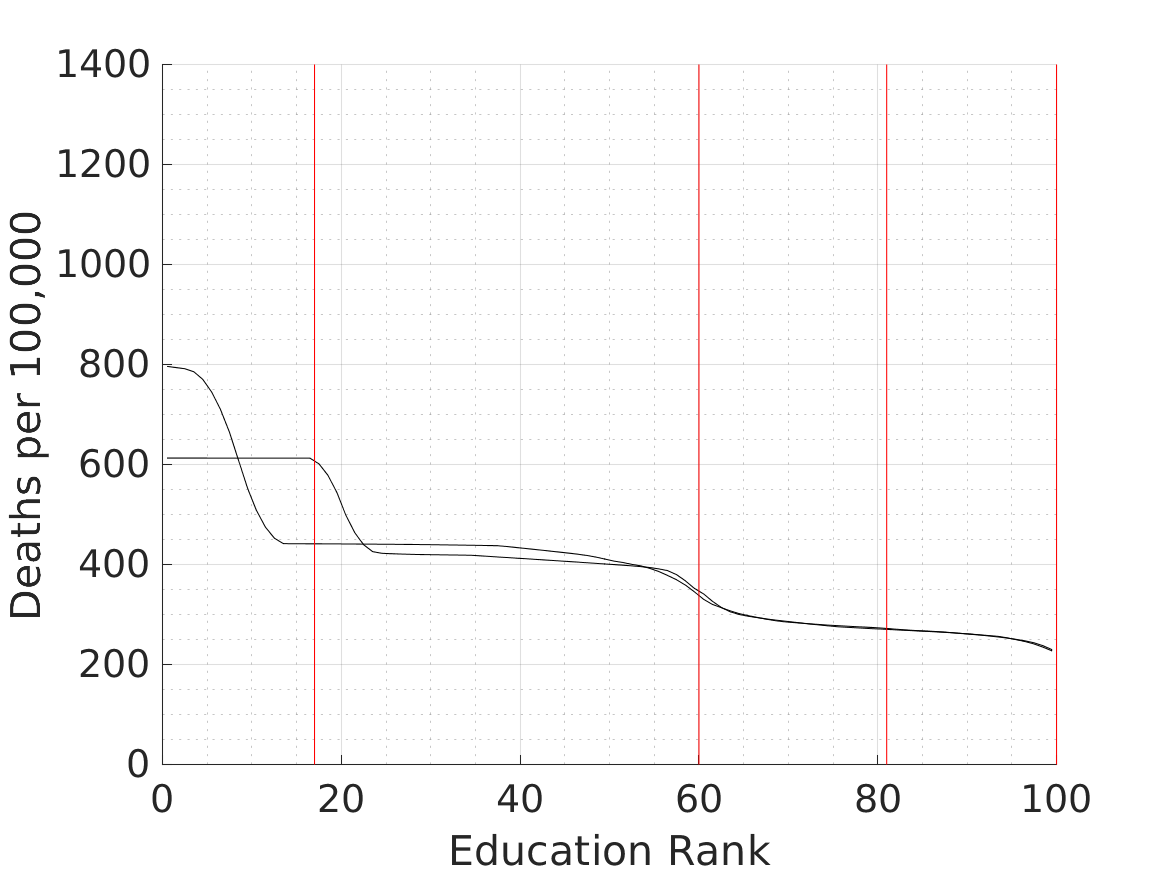
\includegraphics[scale=0.35]{\mortalitypath/f1992_semimon_0.png} &
      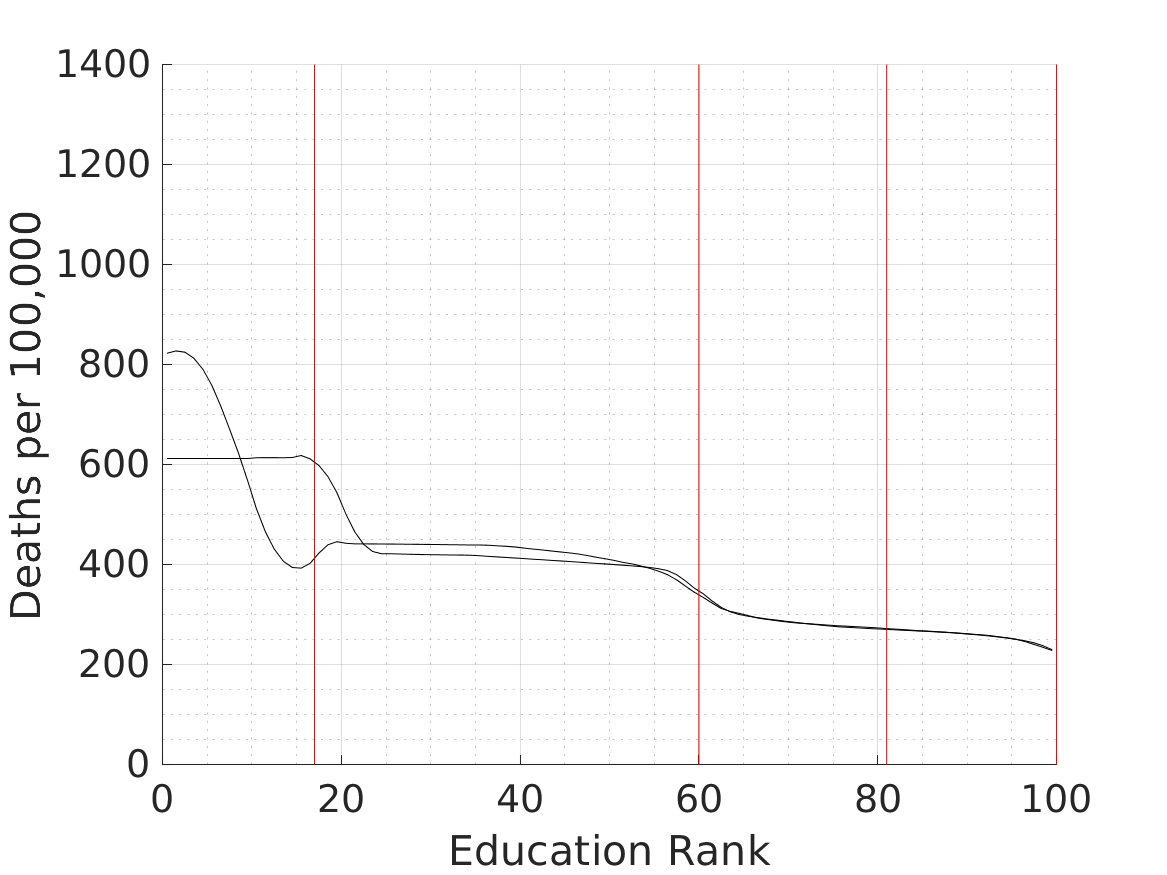
\includegraphics[scale=0.35]{\mortalitypath/f1992_semimon_5.png} \\
      
      \panel\textbf{C. Non-Monotonicity Tolerance = 20} &
      \panel\textbf{D. Non-Monotonicity Tolerance = 100} \\

      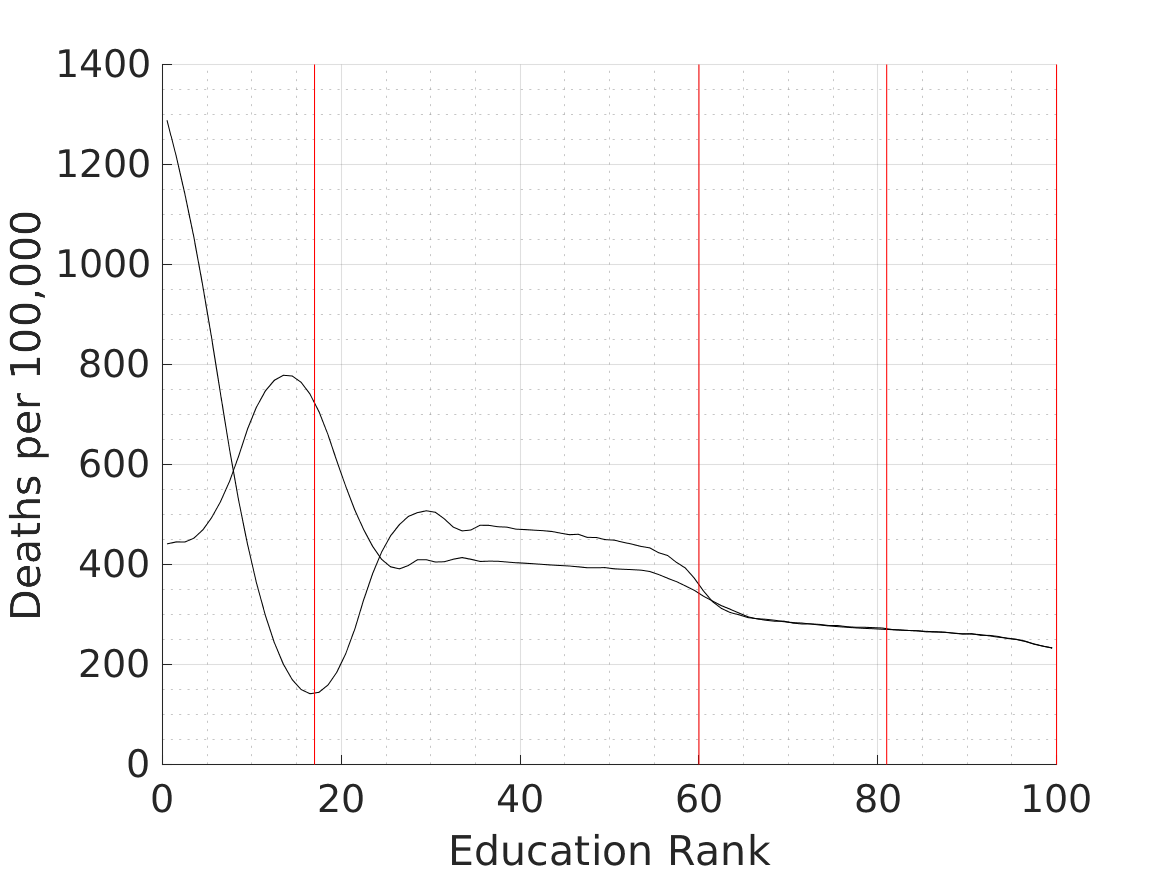
\includegraphics[scale=0.35]{\mortalitypath/f1992_semimon_20.png} &
      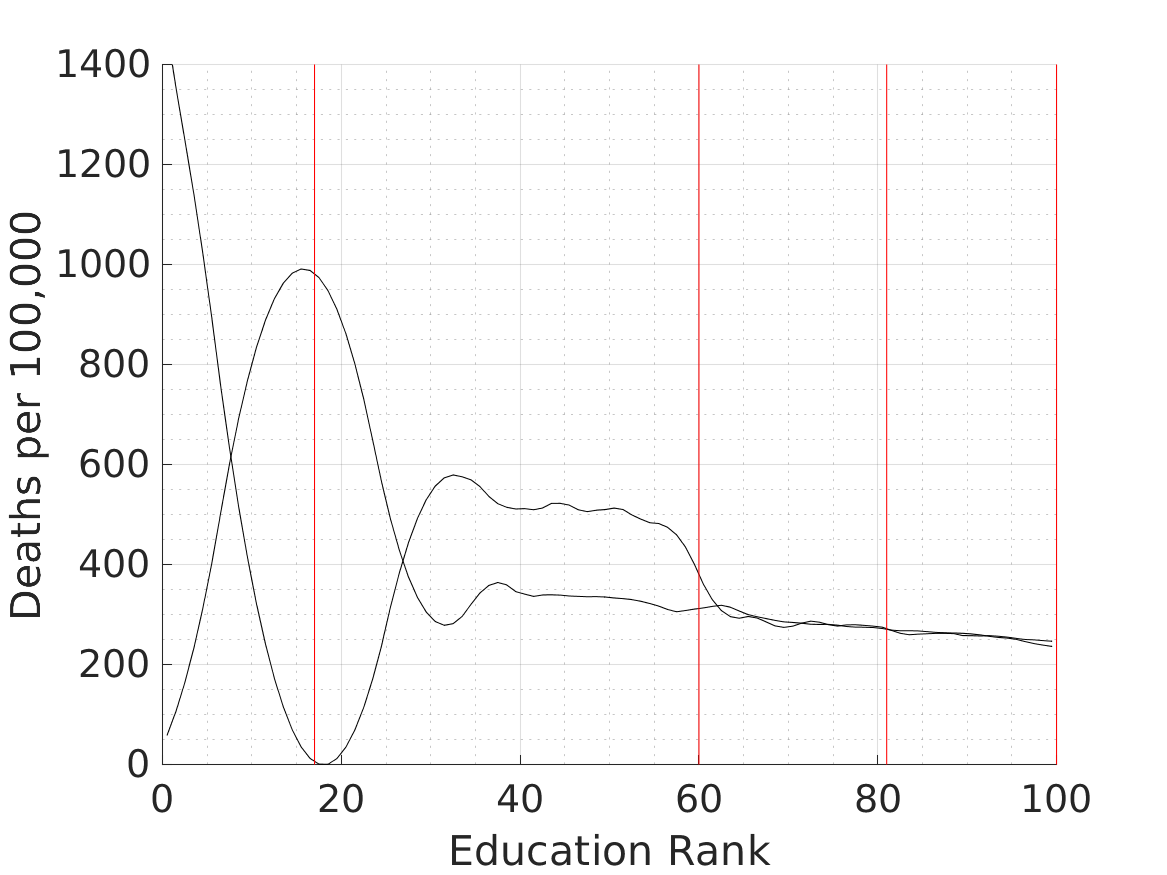
\includegraphics[scale=0.35]{\mortalitypath/f1992_semimon_100.png} \\
      \hline
    \end{tabular}
  \end{center}
  \footnotesize{The figure shows the conditional expectation functions that generate the highest and lowest values of mortality among the least educated 10\%, for 50--54-year-old white women, under different monotonicity assumptions. The tolerance value is the number of rank cells out of 100 where mortality is permitted to be increasing with higher education.}
\end{figure}

